\chapter{Propuesta}

En el presente capítulo se describe la metodología a seguir en esta tesis.
\leonidas{AGREGAR ALGO MÁS LARGO AL FINAL}

Como se muestra en la \autoref{fig:pipeline}, en esta investigación se siguieron los siguientes seis pasos:
(i) preparar simulación, 
(ii) preparar optimización, 
(iii) optimización continua,
(iv) optimización discreta,
(v) optimización de fabricación y
(vi) preparación para fabricación.

Estos pasos se siguieron para optimizar tanto un \emph{bend} como un WDM.
Una vez preparada la simulación, la etapa de optimización (continua, discreta y de fabricación) se realizó
tres veces por cada algoritmo.
La primera ejecución usa un valor de semilla de 128, la segunda de 256 y la tercera de 512.
De esta manera se aseguró iniciar con diseños aleatorios y mantener los resultados reproducibles.
Es importante señalar que los resultados de la optimización continua se usan como punto de inicio
para la optimización discreta. Asimismo, los resultados de la optimización discreta se utilizan como
entrada para la optimización de fabricación.
Este proceso tiene como fin el mantener un buen resultado \citep{Yang2017}.
El valor de $\beta$, presente en la \autoref{eq:topo-smooth}, representa el factor discretizador de nuestros diseños.
Este valor se va incrementando en la optimización discreta y de fabricación como se muestra en la
\autoref{fig:pipeline}.
Finalmente, tras haber conseguido diseños optimizados se realizó un post-procesamiento para dejar los diseños
en un formato listo para fabricación.

En las siguientes subsecciones se explica en detalle cada una de los pasos de la metodología seguida en esta tesis.

\begin{figure}[ht]
  \centering
  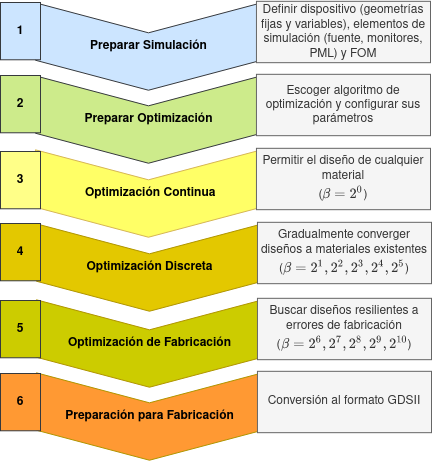
\includegraphics[width=\textwidth]{image/proposal/pipeline.png}
  \caption{Metodología del trabajo de investigación}
  \label{fig:pipeline}
\end{figure}

\section{Preparar Simulación}

El \emph{bend} y WDM se parametrizaron usando la parametrización basada en topología descrita en la
\autoref{sec:parametrization}.
La descripción detallada para los dos dispositivos de estudio se presentan en las siguientes dos subsecciones.

\subsection{\emph{Bend}}

\begin{figure}[ht]
  \centering
  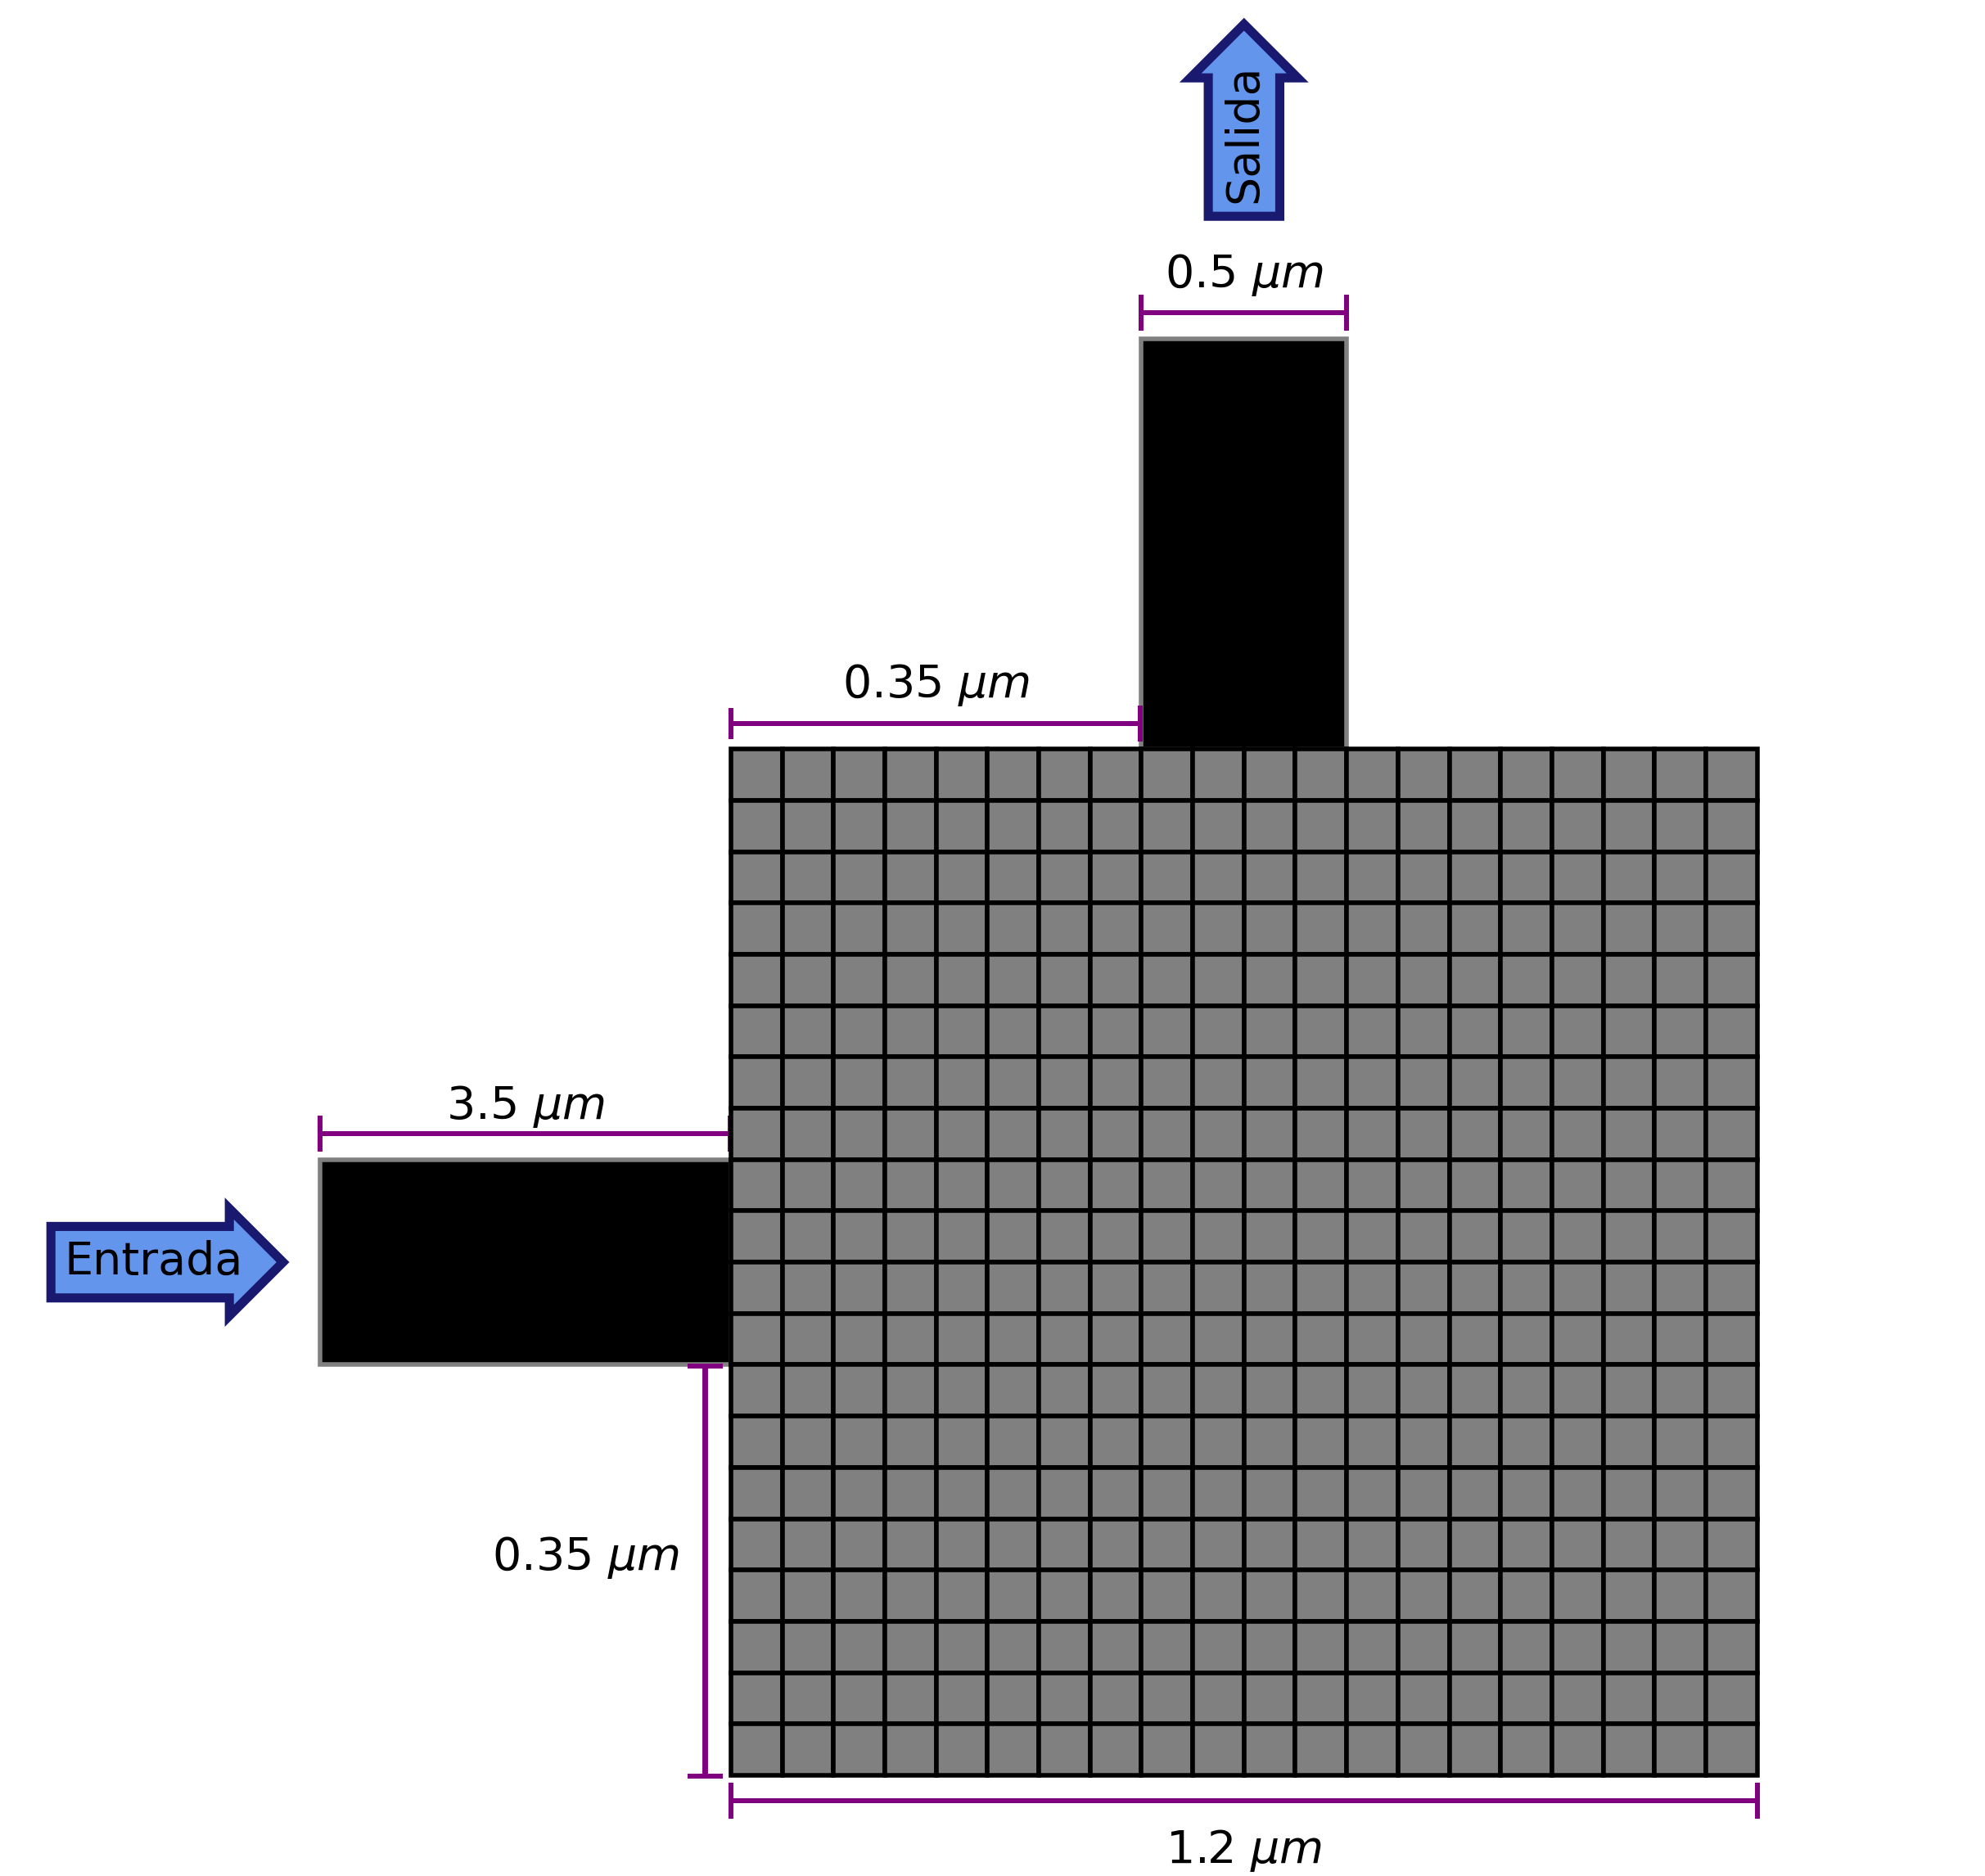
\includegraphics[width=0.7\textwidth]{image/proposal/bend.png}
  \caption{Parámetros del diseño del \emph{bend} a optimizar.}
  \label{fig:dimensiones-bend}
\end{figure}

En la \autoref{fig:dimensiones-bend} se muestra el diseño y parámetros del \emph{bend} a utilizar.
Los rectángulo negros representan las guías de onda, estos tienen las mismas dimensiones aunque en distinta orientación.
La región gris representa la región de diseño.
\leonidas{Al rectángulo con perímetro punteado} se le añadió el valor de $pml\_dist$ en cada dirección
para luego definir el PML con un grosor de valor $pml$.
La recta roja representa la fuente, esta tiene un longitud de valor
$source \times z\_length$, donde $source$ está en el eje Y y $z\_length$ en el eje Z, es decir la fuente está
representada por un rectángulo en YZ.
De manera similar, la recta azul representa el monitor y se encuentra en el eje XZ, este tiene dimensiones
$monitor \times z\_length$. La profundidad de todo es diseño es de $depth$.

Los parámetros fueron escogidos basándonos en \cite{Su2020}.
Primero, la región de diseño se dividió en rectángulos de $16 nm \times 16 nm$.
El valor de los demás parámetros se presenta en la \autoref{tab:bend-values}.

\begin{table}[ht]
    \centering
    \begin{tabular}{|c|c|}
    \hline 
    Parámetro &  Valor (nm) \\
    \hline 
    pml & 300 \\
    pml\_dist & 200 \\
    $d_1$ & 400 \\
    $d_2$ & 400 \\
    L\_width & 2000 \\
    L\_height & 2000 \\
    source & 2500 \\
    monitor & 2500 \\
    z\_length & 1000 \\
    depth & 220 \\
    \hline 
    \end{tabular}
    \caption{\leonidas{Parámetros} usados en el diseño del \emph{bend} a optimizar.}
    \label{tab:bend-values}
\end{table}

\subsection{WDM}

\begin{figure}[ht]
  \centering
  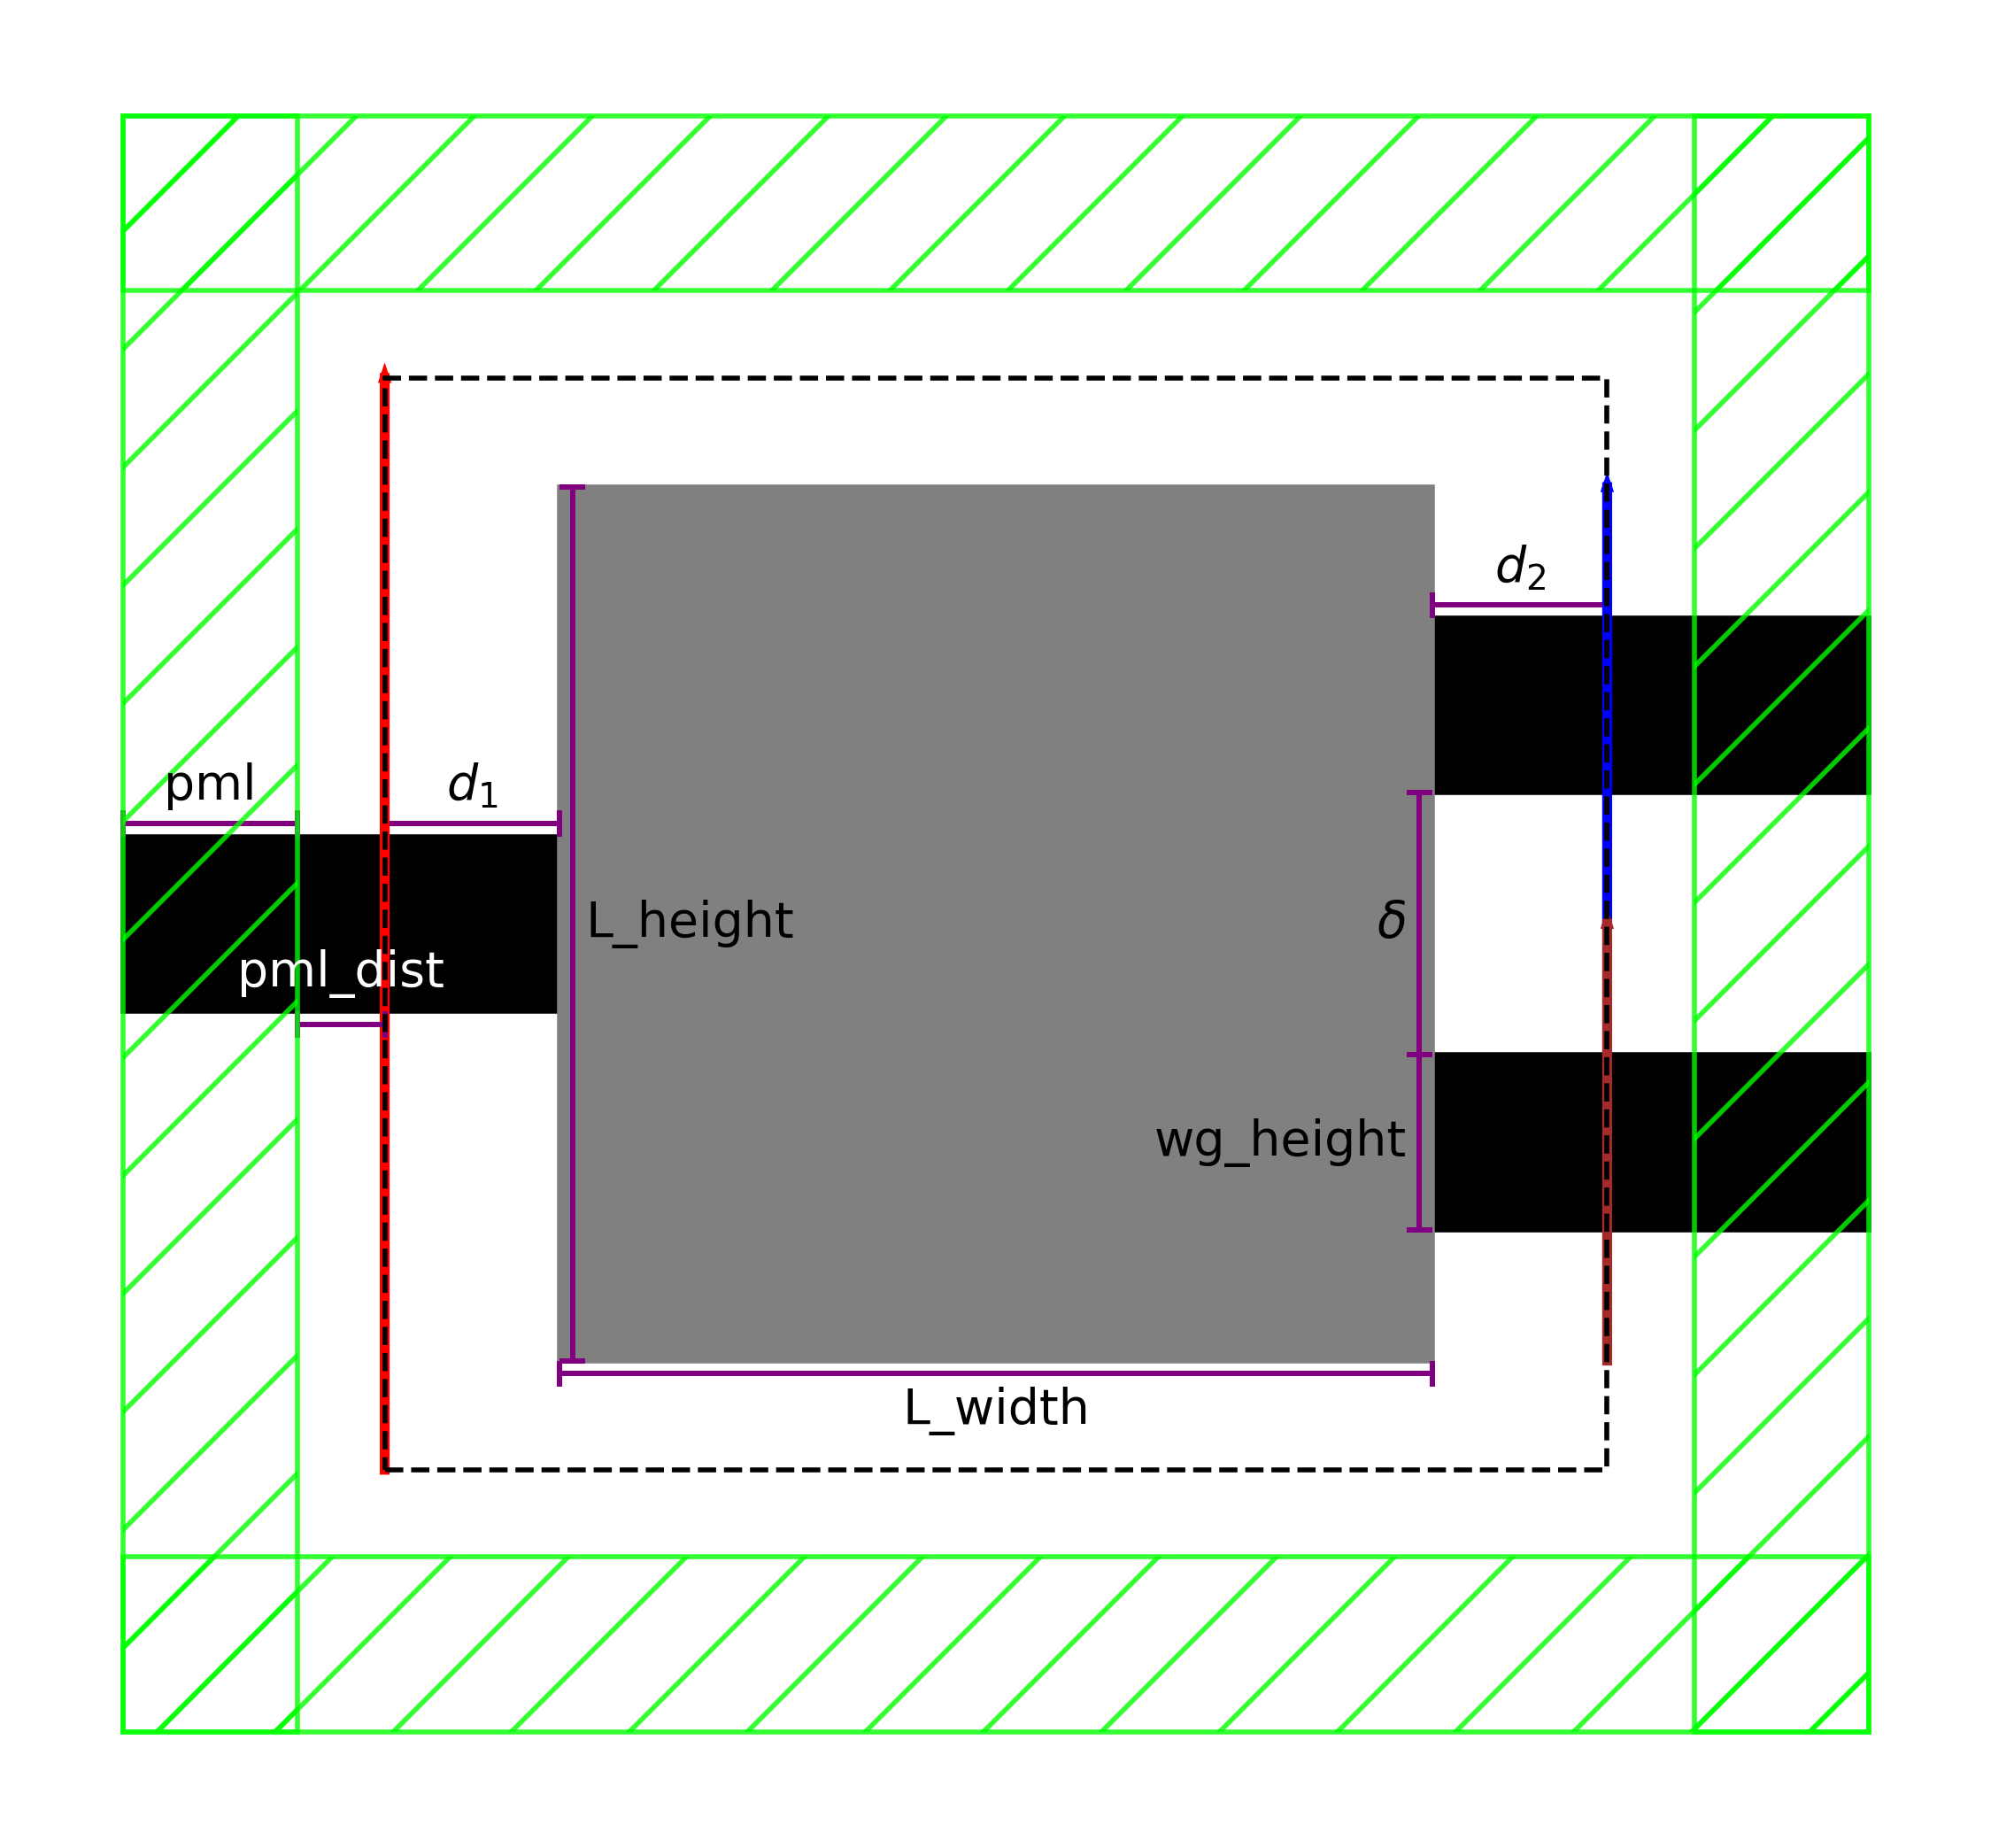
\includegraphics[width=0.8\textwidth]{image/proposal/wdm.png}
  \caption{Parámetros del diseño del \emph{bend} a optimizar.}
  \label{fig:dimensiones-demultiplexer}
\end{figure}

En la figura \ref{fig:dimensiones-demultiplexer} se muestra el diseño y dimensiones del WDM a utilizar.
Los rectángulos negros representas las guías de onda, estos tienen las mismas dimensiones.
La región gris representa la región de diseño, esta región ha sido dividida en una cuadrícula de $20 \times 20$.
Cada píxel tiene $60 nm$ de lado y una permitividad asociada dada por la ecuación \ref{eq:permitivity}.

\section{Función objetivo}

Basándonos en el trabajo de \cite{Su2020}, para el \emph{bend} usaremos como función objetivo la ecuación \ref{eq:fom-bend} y para el WDM la ecuación \ref{eq:fom-splitter}.

\section{Optimización}

El proceso de optimización se dividirá en tres etapas: (i) optimización continua, (ii) optimización discreta y (iii) optimización de fabricación.
Tomando como base a \cite{Elsawy2020, Schneider2019, Gregory2015}, este proceso se realizará con los siguientes cinco algoritmos: (i) L-BFGS-B, (ii) \emph{covariance matrix adaptation evolution strategy} (CMA-ES), (iii) \emph{particle swarm optimization} (PSO), (iv) algoritmos genéticos (GA), (v) optimización bayesiana (OB).

Similar a \cite{Schneider2019}, para poder comparar los resultados el proceso se repetirá 6 veces por cada algoritmo y en cada repetición se fijará el valor de la semilla con el fin de asegurar reproducibilidad de los experimentos.
Además, en cada etapa de la optimización se realizará un cambio de sus parámetros, en la medida de lo posible, para asegurar ir convergiendo a un resultado óptimo.
Adicionalmente, se limitará la cantidad de posibles diseños a simular.
Así se podrá hacer una comparación del desempeño de los algoritmos en base a la cantidad de evaluaciones de la función objetivo.
Sin embargo, debido a que estos algoritmos trabajan de forma iterativa con sus propias particularidades, se considerará como condición de salida el estar en la primera iteración donde ya se haya realizado la cantidad máxima de simulaciones.

A continuación, se describirá las características de cada etapa del proceso de optimización.

\subsubsection{Optimización continua}

En este primer paso se usará directamente la ecuación \ref{eq:permitivity} para buscar dispositivos óptimos de acuerdo al FOM definido.
Así, es probable obtener diseños con muy buenos resultados, pero con permitividades no asociadas al $SiO_2$ o $Si$.
Cada algoritmo comenzará con un diseño inicial aleatorio y se limitará en 5000 la cantidad de posibles diseños a simular. 
Las simulaciones se realizarán en 2D.

\subsubsection{Optimización discreta}

Bajo la premisa que la anterior etapa obtuvo un buen resultado, cada algoritmo tomará como punto inicial el resultado de la optimización previa y tratará de configurar sus parámetros para realizar la búsqueda principalmente alrededor de ese punto.

Además, se aplicará la ecuación \ref{eq:topo-smooth} al parámetro $\lambda$ de la ecuación \ref{eq:permitivity} para gradualmente terminar mapeando al $SiO_2$ o $Si$ en cada píxel. 
Para ello se realizará 5 optimizaciones donde el resultado de una funcionará como punto inicial de la siguiente.
En cada una de estas optimizaciones se limitará en 5000 la cantidad de posibles diseños a simular y se tomará como parámetro $\beta$ de la ecuación \ref{eq:topo-smooth} el valor dado por la siguiente recurrencia:

\begin{equation}
  \begin{split}
    \beta_1 &= 2\\
    \beta_n &= \beta_{n-1} \times 2
  \end{split}
  \label{eq:beta-param}
\end{equation}

Las simulaciones se realizarán en 2D.

\subsubsection{Optimización de fabricación}

Con la anterior etapa la ecuación \ref{eq:topo-smooth} nos asegura diseños que están convergiendo a dispositivos reales.
Ahora, tomando como referencia el trabajo de \cite{Hammond20} para asegurar un buen desempeño pese a los errores de fabricación, por cada parametrización $p$ se calculará:

\begin{itemize}
  \item $p_{ext}$ que representará el diseño como si el dispositivo se hubiera dilatado.
  \item $p_{int}$ que representará el diseño como si el dispositivo se hubiera contraído.
\end{itemize}

Luego, se definirá como nueva función objetivo la siguiente ecuación:

\begin{equation}
  \begin{split}
    F_{obj} &= \omega_1 f^2_{obj}(p) + \omega_2 (1 - |f_{obj}(p_{ext}) - f_{obj}(p_{int})|)^2\\
    \omega_1 &= 0.85\\
    \omega_2 &= 0.15
  \end{split}
  \label{eq:final-fom}
\end{equation}

Así, se buscará un diseño que tenga un buen desempeño y que sea resiliente a posibles errores de fabricación.
Además, para asegurar que los resultados sean más congruentes con la realidad las simulaciones se realizarán en 3D con la ayuda de un GPU.

\subsection{Preparación para fabricación}

Para que nuestros diseños puedan ser fabricados, necesitamos representarlo en formato GDSII.
Para ello, con los mejores resultados de cada algoritmo usaremos la distribución de la permitividad asociada a su parametrización, $\epsilon(p)$,
para obtener la geometría del dispositivo.
Así, nuestra tarea se reducirá a aproximar el contorno de esta geometría con polígonos para luego realizar la conversión al formato GDSII.
Además, usaremos el resultado en formato GDSII para simular el funcionamiento del dispositivo y asegurar que siga manteniendo las propiedades deseadas.
En caso no se tenga éxito, se volverá a iterar en la conversión

\subsection{Fabricación}

Se mandará a fabricar los mejores resultados hasta cubrir el área dispuesta para fabricación. 
Luego, se esperará las mediciones de los dispositivos ya fabricados para compararlo con los resultados de las simulaciones computacionales.
